\section{Use Case Diagram}
\justify
A use case diagram for AyurSpace highlights interactions between the Mobile User,
Plant.id API, and Gemini API---authentication, plant scanning, dosha quiz, and AyurBot
wellness advice.

\begin{figure}[!htbp]
\begin{mdframed}
\centering
\resizebox{\linewidth}{!}{%
\begin{tikzpicture}[>=Stealth, thick, yscale=1.3,
    uc/.style={ellipse, draw, thick, align=center,
               minimum width=3.2cm, minimum height=1.1cm, font=\small},
    lbl/.style={font=\tiny, fill=white, inner sep=1.5pt}]

%% ── System boundary ──────────────────────────────────────────────
\draw[thick] (2.5, 0.5) rectangle (15.5, 13.2);
\draw[thick] (2.5, 12.5) -- (15.5, 12.5);
\node[font=\small\bfseries] at (9.0, 12.85) {AyurSpace Application};

%% ── Mobile User (left) ───────────────────────────────────────────
\draw[thick] (0.7, 8.8)  circle (0.4);
\draw[thick] (0.7, 8.4)  -- (0.7, 7.2);
\draw[thick] (0.3, 7.8)  -- (1.1, 7.8);
\draw[thick] (0.7, 7.2)  -- (0.35, 6.4);
\draw[thick] (0.7, 7.2)  -- (1.05, 6.4);
\node[font=\small, align=center] at (0.7, 6.05) {Mobile\\User};

%% ── Plant.id API (right) ─────────────────────────────────────────
\draw[thick] (16.8, 10.5) circle (0.4);
\draw[thick] (16.8, 10.1) -- (16.8,  8.9);
\draw[thick] (16.4,  9.5) -- (17.2,  9.5);
\draw[thick] (16.8,  8.9) -- (16.45, 8.1);
\draw[thick] (16.8,  8.9) -- (17.15, 8.1);
\node[font=\small, align=center] at (16.8, 7.75) {Plant.id\\API};

%% ── Gemini API (right) ───────────────────────────────────────────
\draw[thick] (16.8, 6.5)  circle (0.4);
\draw[thick] (16.8, 6.1)  -- (16.8,  4.9);
\draw[thick] (16.4, 5.5)  -- (17.2,  5.5);
\draw[thick] (16.8, 4.9)  -- (16.45, 4.1);
\draw[thick] (16.8, 4.9)  -- (17.15, 4.1);
\node[font=\small, align=center] at (16.8, 3.75) {Gemini\\API};

%% ── Primary use cases (left column) ─────────────────────────────
\node[uc] (auth)  at (6.5, 11.5) {Authenticate\\User};
\node[uc] (scan)  at (6.5,  9.8) {Scan Plant\\Image};
\node[uc] (chat)  at (6.5,  8.1) {Chat with\\AyurBot};
\node[uc] (quiz)  at (6.5,  6.4) {Take Dosha\\Quiz};
\node[uc] (hist)  at (6.5,  4.7) {View Scan\\History};
\node[uc] (prof)  at (6.5,  3.0) {Update Profile};

%% ── Secondary use cases (right column) ──────────────────────────
\node[uc, minimum width=2.4cm] (login) at (13.0, 6.2)  {Login};
\node[uc]                      (ident) at (11.0, 9.8)  {Identify Plant\\Taxonomy};
\node[uc]                      (fetch) at (11.0, 8.1)  {Fetch Ayurvedic\\Info};

%% ── Mobile User → primary use cases ─────────────────────────────
\draw[->] (1.1, 7.8) -- (auth.west);
\draw[->] (1.1, 7.8) -- (scan.west);
\draw[->] (1.1, 7.8) -- (chat.west);
\draw[->] (1.1, 7.8) -- (quiz.west);
\draw[->] (1.1, 7.8) -- (hist.west);
\draw[->] (1.1, 7.8) -- (prof.west);

%% ── auth → login: L-shaped to avoid crossing ident/fetch ────────
\draw[->, dashed] (auth.east) -| (login.north);
\node[lbl] at (10.5, 11.6) {$\langle\!\langle$include$\rangle\!\rangle$};

%% ── chat / quiz / hist / prof → login (direct dashed) ───────────
\draw[->, dashed] (chat.east) --
    node[lbl, above, pos=0.5] {$\langle\!\langle$include$\rangle\!\rangle$}
    (login.west);
\draw[->, dashed] (quiz.east) --
    node[lbl, above, pos=0.5] {$\langle\!\langle$include$\rangle\!\rangle$}
    (login.west);
\draw[->, dashed] (hist.east) --
    node[lbl, below, pos=0.5] {$\langle\!\langle$include$\rangle\!\rangle$}
    (login.south west);
\draw[->, dashed] (prof.east) to[out=0, in=240]
    node[lbl, below right, pos=0.55] {$\langle\!\langle$include$\rangle\!\rangle$}
    (login.south);

%% ── scan → ident (<<include>>) ───────────────────────────────────
\draw[->, dashed] (scan.east) --
    node[lbl, above] {$\langle\!\langle$include$\rangle\!\rangle$}
    (ident.west);

%% ── ident → fetch (<<extend>>) ───────────────────────────────────
\draw[->, dashed] (ident.south) --
    node[lbl, right] {$\langle\!\langle$extend$\rangle\!\rangle$}
    (fetch.north);

%% ── use cases → external actors ─────────────────────────────────
\draw[->] (ident.east) -- (16.4, 9.5);   %% → Plant.id API arm
\draw[->] (fetch.east) -- (16.4, 5.5);   %% → Gemini API arm

\end{tikzpicture}%
}
\end{mdframed}
\caption{Use Case Diagram}
\end{figure}

\newpage
\subsection{Use Case Document}
\begin{enumerate}
    \item \textbf{User Registration / Authentication:}\\
    Firebase Authentication + Firestore profile sync for cross-device persistence.

    \item \textbf{Scan Medicinal Plant:}\\
    Camera capture $\rightarrow$ local compression $\rightarrow$ Plant.id REST API
    $\rightarrow$ taxonomic identity and health assessment.

    \item \textbf{Consult AyurBot:}\\
    Dynamic prompts inject user's \textit{Dosha} profile + conversation history into
    Gemini LLM for hyper-personalized responses.

    \item \textbf{Tridosha Questionnaire:}\\
    Algorithmic scoring of Vata/Pitta/Kapha questions generates user's \textit{Prakriti}.

    \item \textbf{Image Pre-processing (Internal):}\\
    Bicubic downsampling converts 12MP captures to compressed Base64 byte arrays,
    reducing API latency and ensuring stability.
\end{enumerate}

\newpage
\section{Class Diagram}
The class diagram adheres to UML~2.x conventions. Classes are colour-coded by
stereotype: \textit{service} (blue) for external-API wrappers, \textit{entity}
(green) for persistent domain objects, \textit{value~object} (purple) for
immutable data carriers, and \textit{state} (amber) for Riverpod notifier state.
Visibility markers follow UML notation: ($-$) denotes private and
($+$) denotes public. Dashed arrows represent dependencies; solid arrows
represent associations; a hollow diamond at the source denotes aggregation.

\begin{figure}[!htbp]
  \begin{mdframed}
    \centering
    \resizebox{\linewidth}{!}{%
    \begin{tikzpicture}[>=Stealth,
        %% ── Stereotype-coloured UML class styles ──────────────────────────
        cls/.style={
            rectangle split, rectangle split parts=3,
            draw=black!70, line width=0.8pt,
            rectangle split part align={center, left, left},
            inner sep=5pt, font=\small
        },
        svc/.style={cls, rectangle split part fill={SteelBlue!35,  white, white}},
        ent/.style={cls, rectangle split part fill={ForestGreen!30, white, white}},
        val/.style={cls, rectangle split part fill={Plum!20,        white, white}},
        sta/.style={cls, rectangle split part fill={Goldenrod!40,   white, white}},
        %% ── Relationship arrow styles ──────────────────────────────────────
        assoc/.style={-{Stealth[length=6pt,width=4pt]}, thick},
        dep/.style  ={-{Stealth[length=6pt,width=4pt]}, dashed, thick},
        agg/.style  ={{Diamond[open,length=9pt,width=5pt]}-{Stealth[length=6pt,width=4pt]}, thick},
        %% ── Relationship label ─────────────────────────────────────────────
        lbl/.style={font=\scriptsize\itshape, fill=white, inner sep=2pt}
    ]

    %% ─── ROW 1: SERVICES ──────────────────────────────────────────────────
    \node[svc, text width=8.5cm] (pis) at (4, 16) {
        \textit{$\ll$service$\gg$}\\\bfseries PlantIdService
        \nodepart{two}
        $-$ \_apiKey : String
        \nodepart{three}
        $+$ identifyFromBytes(bytes : Uint8List)\\
        \quad : Future$<$PlantIdResult$>$
    };

    \node[svc, text width=10.5cm] (gs) at (17, 16) {
        \textit{$\ll$service$\gg$}\\\bfseries GeminiService
        \nodepart{two}
        $-$ \_apiKey : String
        \nodepart{three}
        $+$ getAyurvedicInfo(name : String) : Future$<$GeminiResponse$>$\\[3pt]
        $+$ sendChat(msg : String, history : List$<$ChatTurn$>$)\\
        \quad : Future$<$GeminiResponse$>$
    };

    %% ─── ROW 2: ENTITIES AND VALUE OBJECTS ────────────────────────────────
    \node[val, text width=6cm] (pir) at (1, 9) {
        \textit{$\ll$value object$\gg$}\\\bfseries PlantIdResult
        \nodepart{two}
        $-$ scientificName : String\\
        $-$ commonName : String\\
        $-$ probability : double\\
        $-$ isHealthy : bool\\
        $-$ description : String
        \nodepart{three}
        $+$ fromJson(json : Map) : PlantIdResult
    };

    \node[ent, text width=5cm] (u) at (8.5, 9) {
        \textit{$\ll$entity$\gg$}\\\bfseries User
        \nodepart{two}
        $-$ uid : String\\
        $-$ name : String\\
        $-$ email : String\\
        $-$ dosha : DoshaResult
        \nodepart{three}
        $+$ fromJson(json : Map) : User\\
        $+$ toJson() : Map\\
        $+$ copyWith(\ldots) : User
    };

    \node[ent, text width=5.5cm] (p) at (15.5, 9) {
        \textit{$\ll$entity$\gg$}\\\bfseries Plant
        \nodepart{two}
        $-$ id : String\\
        $-$ scientificName : String\\
        $-$ hindiName : String\\
        $-$ uses : List$<$String$>$\\
        $-$ rasa : String\\
        $-$ virya : String
        \nodepart{three}
        $+$ fromJson(json : Map) : Plant\\
        $+$ toJson() : Map
    };

    \node[val, text width=4.5cm] (gr) at (22, 9) {
        \textit{$\ll$value object$\gg$}\\\bfseries GeminiResponse
        \nodepart{two}
        $-$ text : String\\
        $-$ isError : bool
        \nodepart{three}
        \strut
    };

    %% ─── ROW 3: STATE AND MESSAGES ────────────────────────────────────────
    \node[sta, text width=5.5cm] (cs) at (9, 2) {
        \textit{$\ll$state$\gg$}\\\bfseries ChatState
        \nodepart{two}
        $-$ messages : List$<$ChatMessage$>$\\
        $-$ isTyping : bool\\
        $-$ error : String
        \nodepart{three}
        $+$ copyWith(\ldots) : ChatState
    };

    \node[val, text width=4.5cm] (cm) at (17, 2) {
        \textit{$\ll$value object$\gg$}\\\bfseries ChatMessage
        \nodepart{two}
        $-$ role : String\\
        $-$ content : String
        \nodepart{three}
        \strut
    };

    %% ─── RELATIONSHIPS ────────────────────────────────────────────────────

    %% PlantIdService ..> PlantIdResult  -- straight diagonal down-left
    \draw[dep] (pis.south) --
        node[lbl, sloped, above, midway]{$\ll$creates$\gg$}
        (pir.north);

    %% GeminiService ..> GeminiResponse  -- straight near-vertical from lower-right corner
    \draw[dep] (gs.south east) --
        node[lbl, right, midway]{$\ll$returns$\gg$}
        (gr.north);

    %% GeminiService ..> Plant  -- straight diagonal down-left from bottom centre
    \draw[dep] (gs.south) --
        node[lbl, sloped, above, midway]{$\ll$enriches$\gg$}
        (p.north);

    %% User ──> Plant  saves  0..*
    \draw[assoc] (u.east) --
        node[lbl, above]{saves \quad 0..*}
        (p.west);

    %% ChatState <>── ChatMessage  messages  1..*
    \draw[agg] (cs.east) --
        node[lbl, above]{messages \quad 1..*}
        (cm.west);

    \end{tikzpicture}%
    }
  \end{mdframed}
  \caption{UML Class Diagram --- AyurSpace System}
\end{figure}

\newpage
\section{Activity Diagram}
The activity diagram captures the plant scanning flow: Dashboard $\rightarrow$ Camera
$\rightarrow$ Compress $\rightarrow$ Plant.id API. If confidence $< 0.2$, error/retry.
Otherwise $\rightarrow$ Gemini API $\rightarrow$ Firestore $\rightarrow$ UI render.

\begin{figure}[H]
\begin{mdframed}
    \centering
    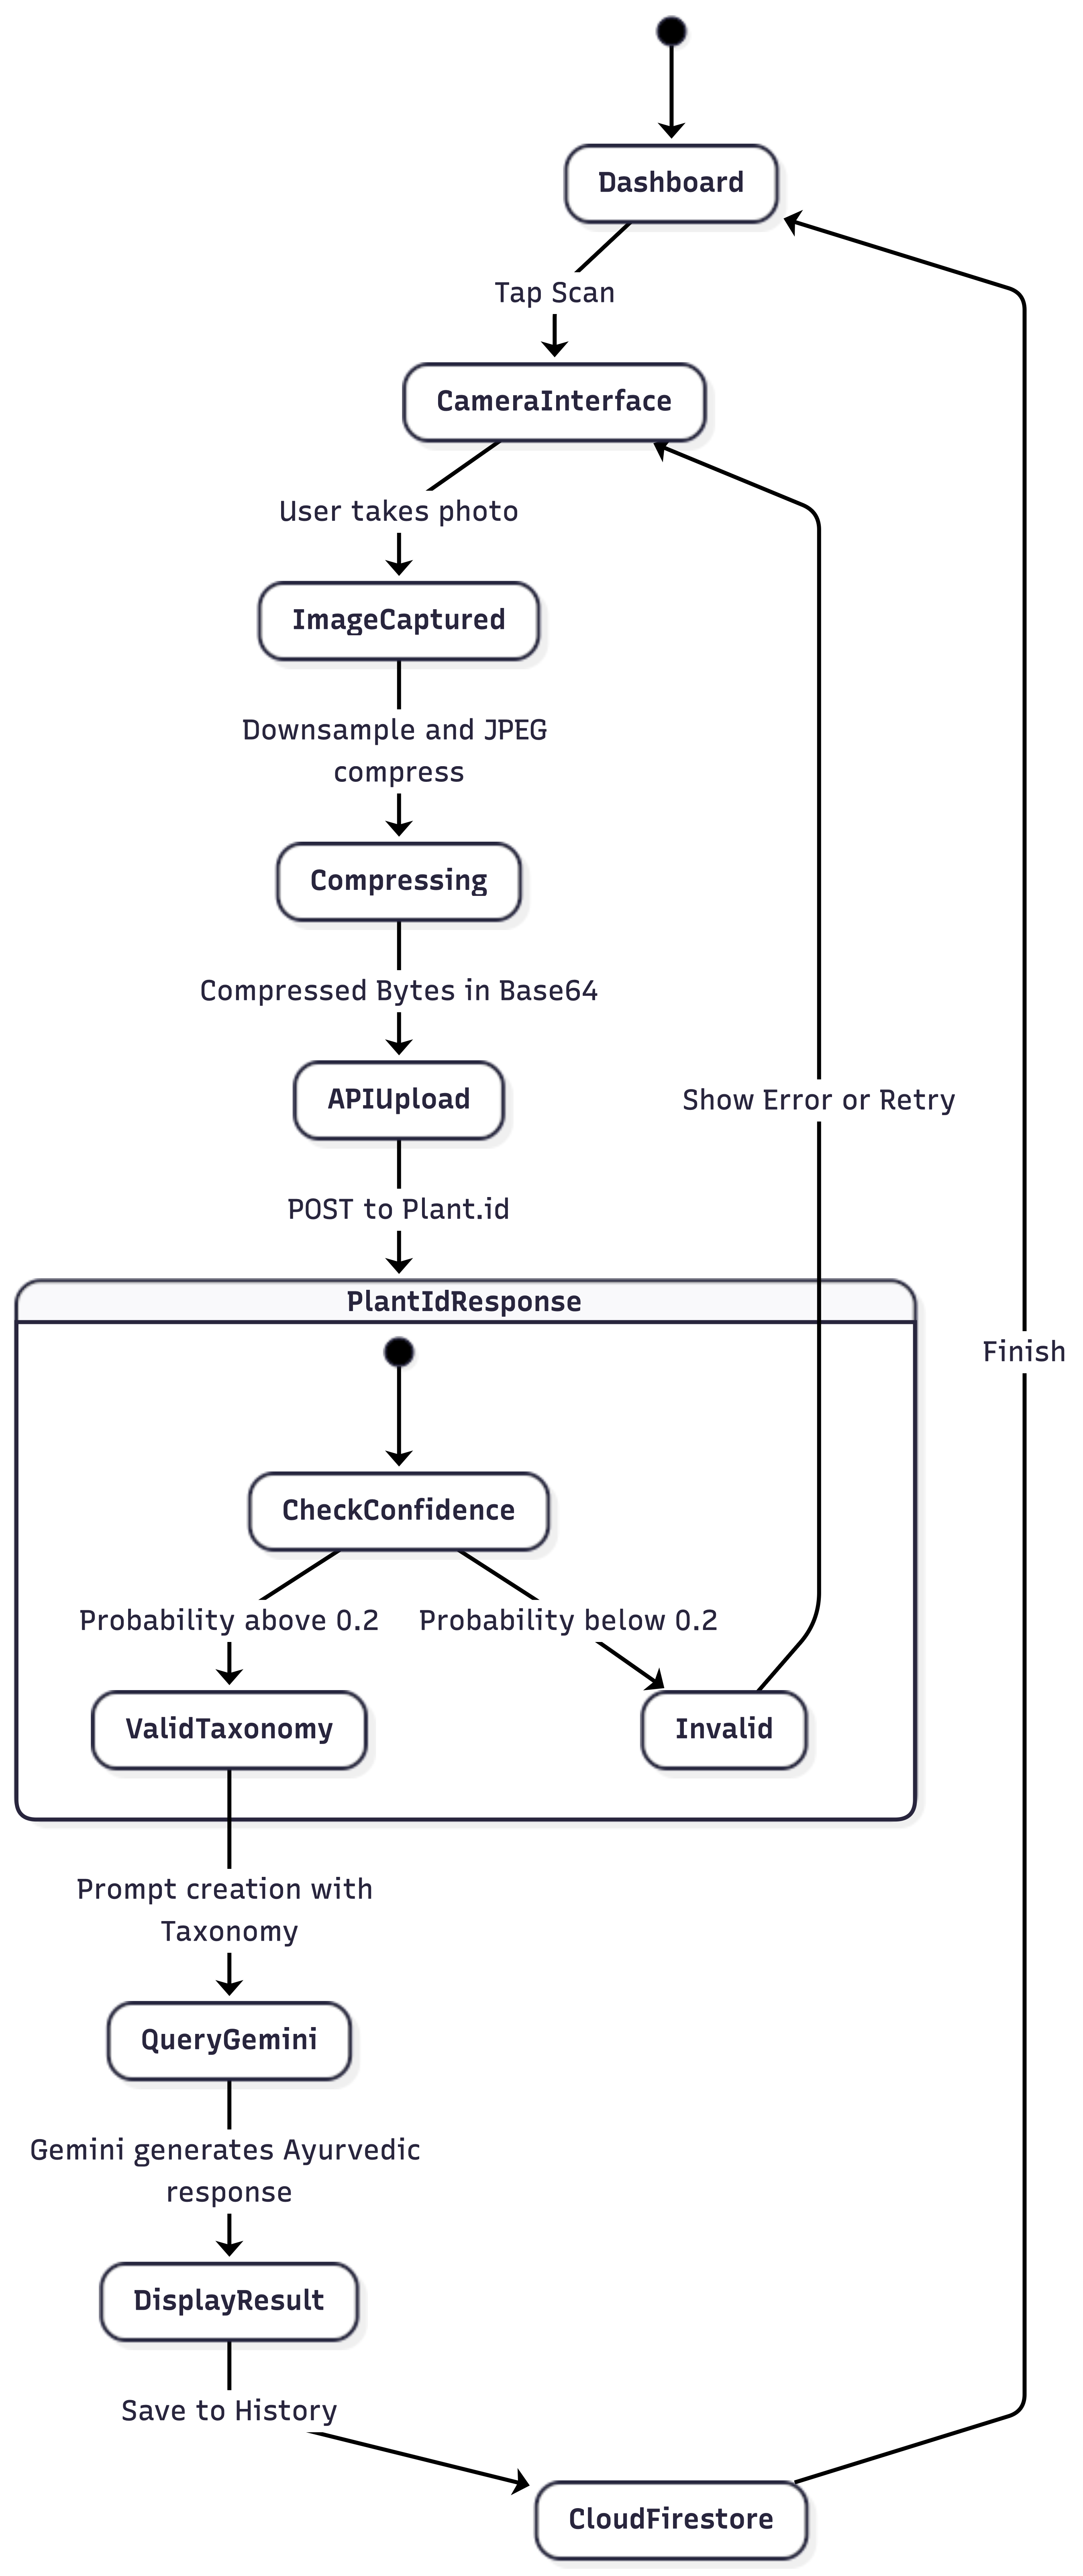
\includegraphics[width=0.5\linewidth, height=0.72\textheight, keepaspectratio]{assets/placeholders/placeholder_activity.png}
\end{mdframed}
    \caption{Activity Diagram}
\end{figure}

\newpage
\section{Sequence Diagram}
\justify
The Sequence Diagram outlines the full execution timeline: Flutter Client $\rightarrow$
POST to Plant.id $\rightarrow$ taxonomy result $\rightarrow$ Gemini API prompt
$\rightarrow$ JSON response $\rightarrow$ Firestore async write $\rightarrow$ UI
dashboard update.

\begin{figure}[!htbp]
\begin{mdframed}
     \centering
    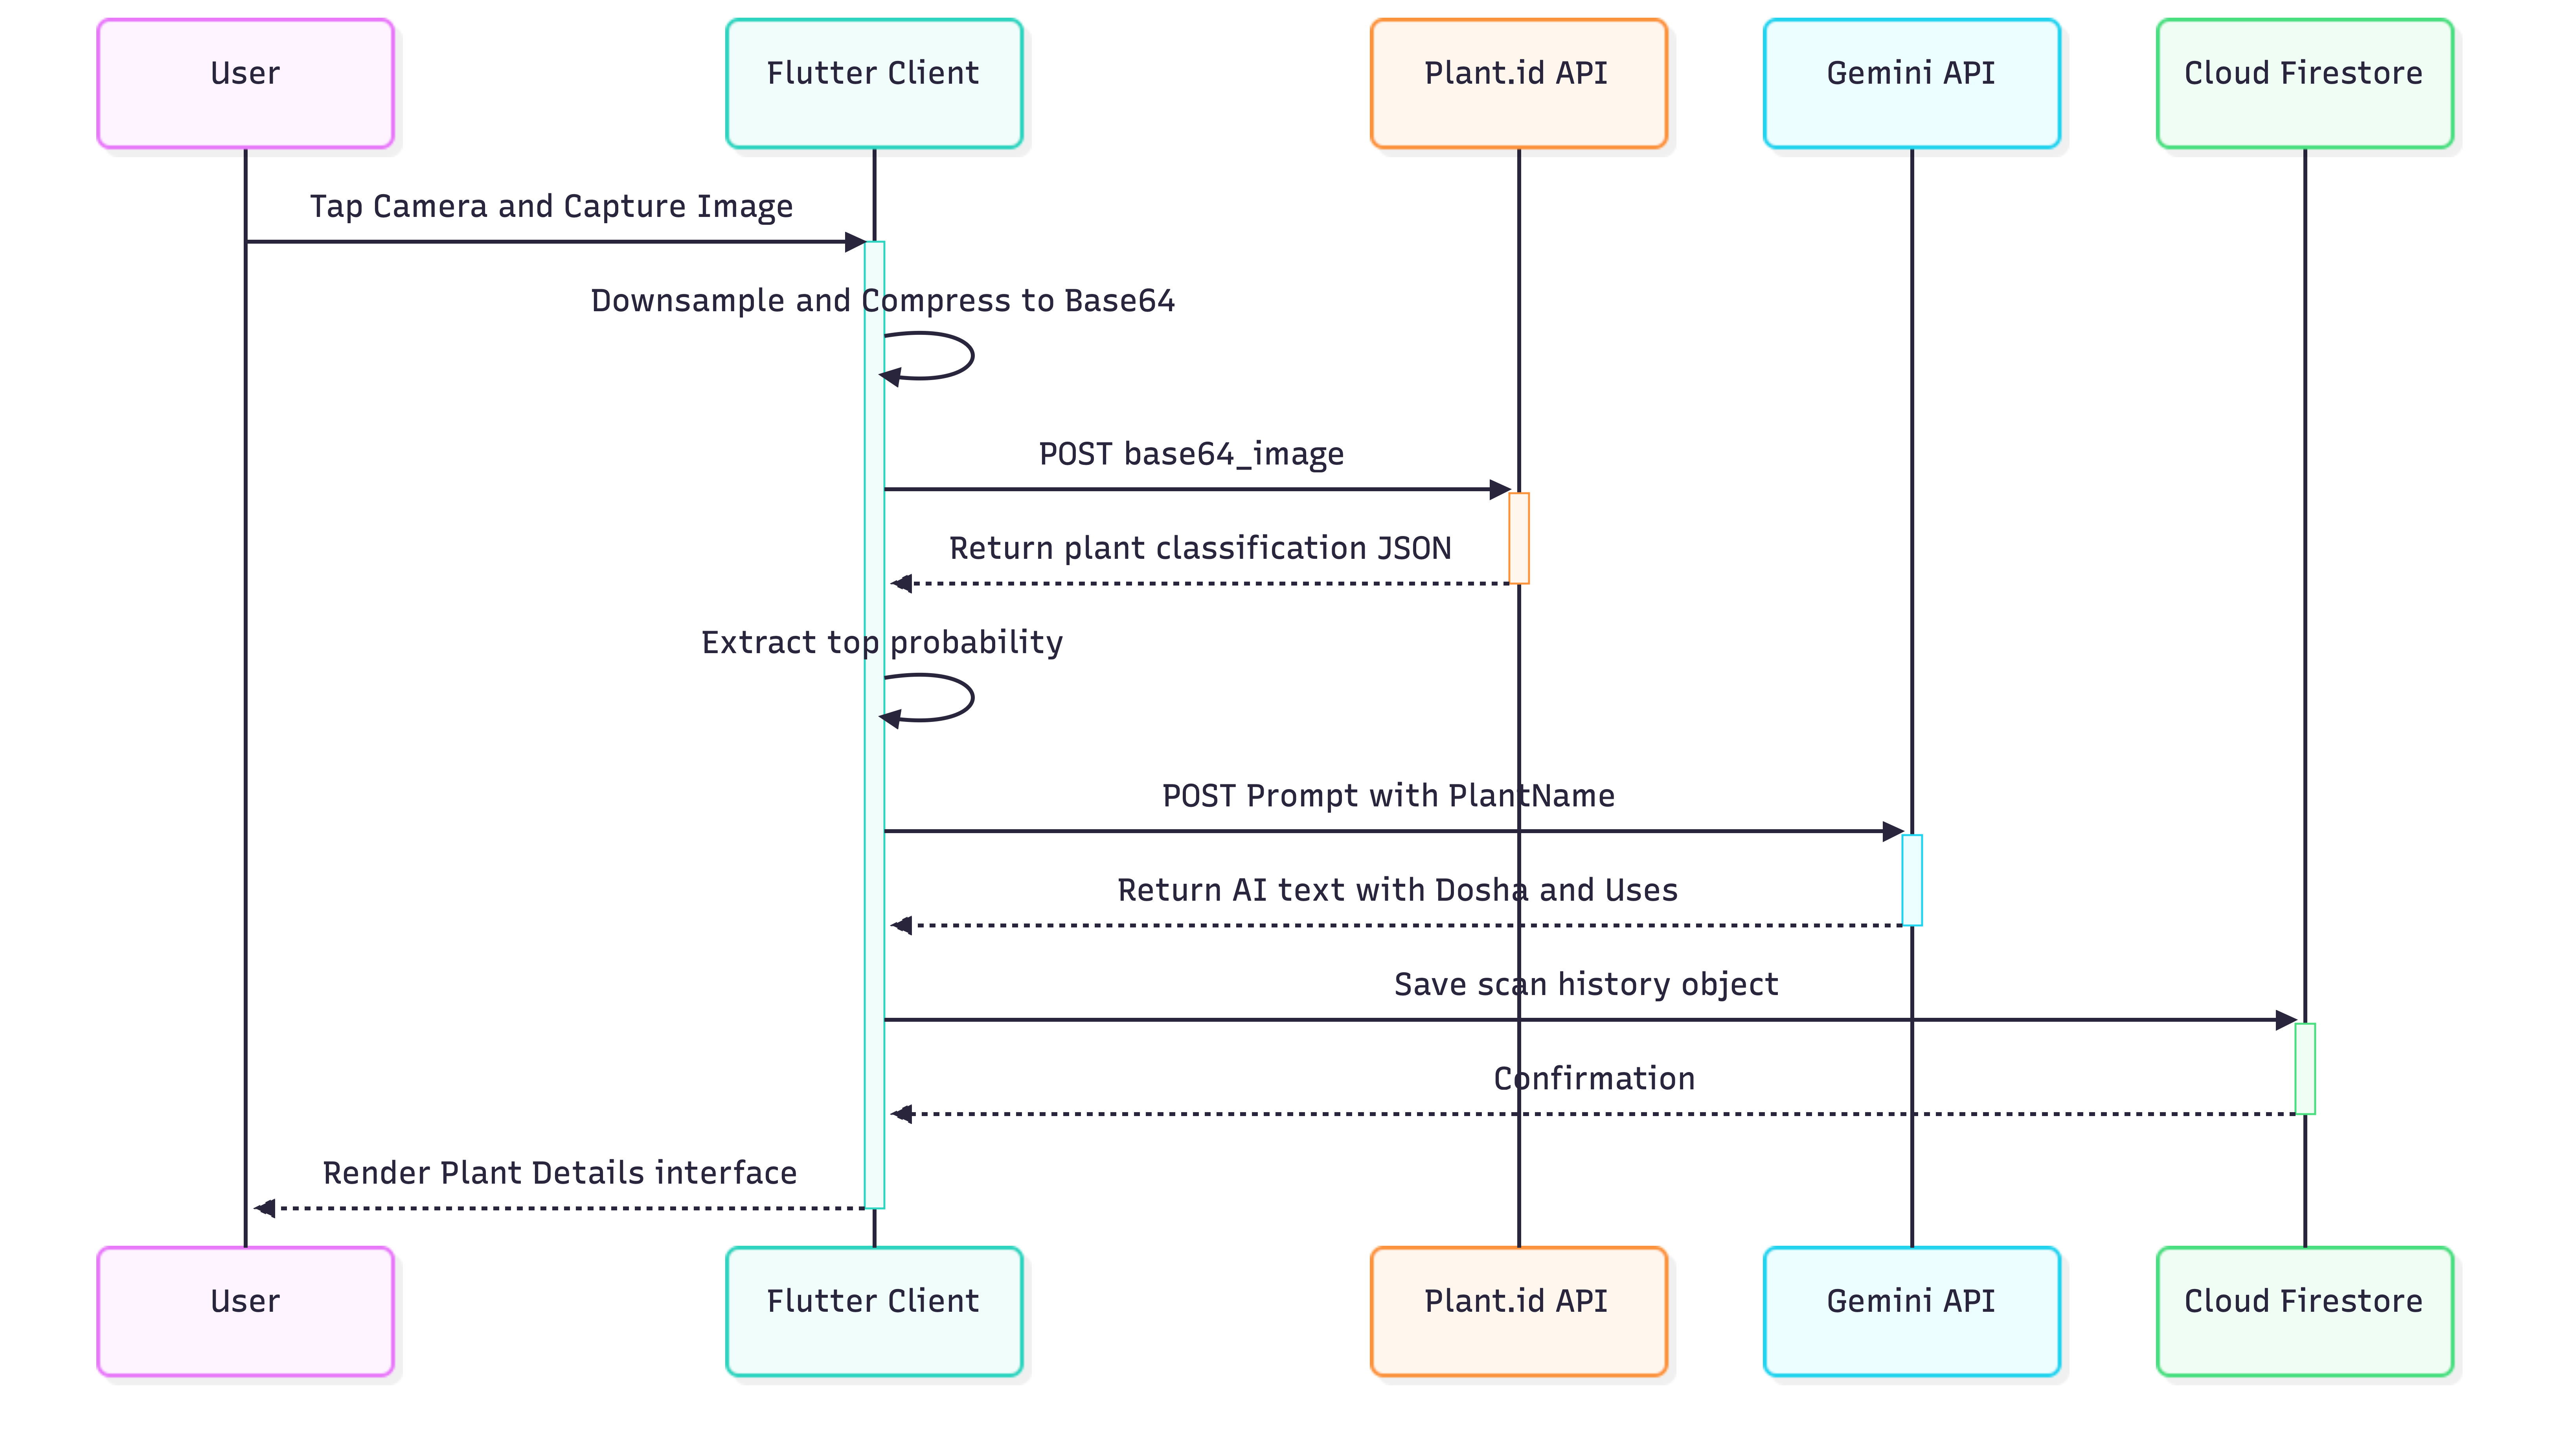
\includegraphics[width=0.84\linewidth,height=0.6\textheight]{assets/placeholders/placeholder_sequence.png}
\end{mdframed}
    \caption{Sequence Diagram}
\end{figure}
